\pdfminorversion=4
\documentclass[10pt]{beamer}
%% O comando acima foi necessario porque o PDF nao abria no acrobat do
%% windows, dava o erro 131. Provavelmente devido as figuras em
%% PDF. Agora ele gera um PDF versao 1.4, ao inves da versao 1.5

\usetheme[compress]{PaloAlto}
\usecolortheme{sidebartab} % crane

\usepackage[brazilian]{babel}
\usepackage[T1]{fontenc}
\usepackage[utf8]{inputenc}
\usepackage{graphicx}
\usepackage{hyperref}
\usepackage[scaled]{beramono} % truetype: Bistream Vera Sans Mono
%\usepackage{inconsolata}
\usepackage{xfrac}
\usepackage{tikz}
\usepackage{xcolor}

\setbeamertemplate{footline}[frame number] % mostra o numero dos slides
\setbeamertemplate{navigation symbols}{} % retira a barra de navegacao

\usepackage{xspace}
\providecommand{\eg}{\textit{e.g.}\xspace}
\providecommand{\ie}{\textit{i.e.}\xspace}
\providecommand{\R}{\textsf{R}\xspace}
\newcommand{\mb}[1]{\mathbf{#1}}
\newcommand{\bs}[1]{\boldsymbol{#1}}
\providecommand{\E}{\text{E}}
\providecommand{\Var}{\text{Var}}
\theoremstyle{definition}
\newtheorem*{mydef}{Definição}
\newtheorem*{mythm}{Teorema}

\title{Introdução à Estatística e conceitos de amostragem}
\author[]{Fernando de Pol Mayer}
\institute[UFPR]{Laboratório de Estatística e Geoinformação (LEG) \\
  Departamento de Estatística (DEST) \\
  Universidade Federal do Paraná (UFPR)}
\date{}
\logo{
\includegraphics[width=1.6cm]{../img/ufpr-logo.png}}
\titlegraphic{
\includegraphics[width=1cm]{../img/CC_by-nc-sa_88x31.png}\\
  \tiny
  \href{https://creativecommons.org/licenses/by-nc-sa/4.0/deed.pt_BR}{Este
    conteúdo está disponível por meio da Licença Creative Commons 4.0
    (Atribuição/NãoComercial/PartilhaIgual)}}

\AtBeginSection[]
{
  \begin{frame}
    \frametitle{Plano de aula}
    \tableofcontents[currentsection]
  \end{frame}
}

\AtBeginSubsection[]
{
  \begin{frame}
    \frametitle{Plano de aula}
    \tableofcontents[currentsection,currentsubsection]
  \end{frame}
}

\begin{document}

\begin{frame}
\maketitle
%\titlepage
\end{frame}

\begin{frame}{Plano de aula}
\tableofcontents
\end{frame}

\section[Estatística]{Estatística}

\subsection[O que é?]{O que é Estatística?}

\begin{frame}{O que é Estatística?}
  \begin{itemize}
  \item Etimologia da palavra: do latim \textit{status} $\Rightarrow$
    estado
  \item Origem: coleta e apresentação de dados de interesse do Estado
    \begin{itemize}
    \item Informações sobre populações e riquezas
    \item Fins militares e tributários
    \end{itemize}
  \item Conjunto de métodos especialmente apropriado ao tratamento de
    dados numéricos, afetados por uma multiplicidade de causas
  \item Estes métodos \textbf{fazem uso} da Matemática, e especialmente
    do cálculo de \textbf{probabilidades}
  \end{itemize}
\end{frame}

\begin{frame}{Um pouco de história \ldots}
  \begin{itemize}
  \item Confúcio relatou levantamentos feitos na China há mais de 2000
    anos AC
  \item No Egito antigo, os faraós fizeram uso sistemático de
    informações de caráter estatístico
  \item O mesmo aconteceu com antigas civilizações como Maias, Astecas e
    Incas
  \item Imperadores faziam levantamentos de suas propriedades
    conquistadas (imperadores romanos, Carlos Magno, Guilherme, o
    Conquistador) para se inteirar de suas riquezas
  \item Essa prática tem sido continuada nos tempos modernos, por meio
    de recenseamentos, como aqueles feitos pelo IBGE no Brasil
  \end{itemize}
\end{frame}

\begin{frame}{O que é Estatística?}
Como Ciência
\begin{itemize}
\item Permite organizar, descrever, analisar, e interpretar dados
\item Utiliza-se da \textbf{Teoria da Probabilidade} para modelar a
  aleatoriedade e a incerteza associada aos fenômenos naturais,
  econômicos, sociais, \ldots
\item Auxilia a tirar \textbf{conclusões} sobre as características das
  fontes de onde os dados foram retirados, para melhor compreende-los
\item Indispensável para a \textbf{tomada de decisões} sob condições de
  \textsl{incerteza}, sob o menor \textbf{risco} possível
\end{itemize}
\end{frame}

\begin{frame}{O que é Estatística?}
Como tecnologia
\begin{itemize}
\item Permite avaliar as incertezas e os seus efeitos no planejamento e
  interpretação de experiências e de observações de fenômenos da
  natureza e da sociedade
\item Permite analisar e tirar conclusões de uma grande quantidade de
  informações
\item A estatística tem sido utilizada para
  \begin{itemize}
  \item Otimização de recursos econômicos
  \item Aumento da qualidade e produtividade
  \item Análise de decisões judiciais
  \item Previsões (climáticas, econômicas, \ldots)
  \end{itemize}
\end{itemize}
\end{frame}

\subsection[Por que?]{Por que estudar Estatística?}

\begin{frame}{Por que estudar Estatística?}
  \begin{itemize}
  \item Impossibilidade de estudar a população
  \item Aumento da capacidade de registro de dados que precisam ser
    compreendidos
  \item Expansão do conhecimento científico, das áreas de pesquisa e dos
    instrumentos de investigação
  \item Necessidade de compreensão dos fenômenos naturais e sociais, de
    otimização de recursos, planejamento de atividades, redução de riscos,
    de previsão de resultados para correta tomada de decisão
  \end{itemize}
\end{frame}

\begin{frame}{Por que estudar Estatística?}
  A Estatística pode ser pensada como a \textbf{ciência de aprendizagem
    a partir dos dados} \\~\\
  Vivemos na ``\textit{era da informação}'', e a Estatística possui as
  ferramentas necessárias para melhor compreender a \textbf{informação}
\end{frame}

\subsection[Computadores]{Estatística e o uso de computadores}

\begin{frame}{Estatística e o uso de computadores}
  No passado, tratar um grande conjunto de dados era uma tarefa
  trabalhosa e cansativa \\~\\

  Com o avanço da tecnologia, os cálculos se tornaram rápidos e
  mecânicos, possibilitando a analise de um volume grande de informações
  em pouco tempo \\~\\

  No entanto, é necessário \textit{conhecer} e \textit{compreender} os
  conceitos básicos de Estatística para que possamos utiliza-la de forma
  adequada
\end{frame}

\subsection[Áreas]{Áreas da Estatística}

\begin{frame}{Organograma da Estatística}
  \begin{figure}[h]
    \centering
    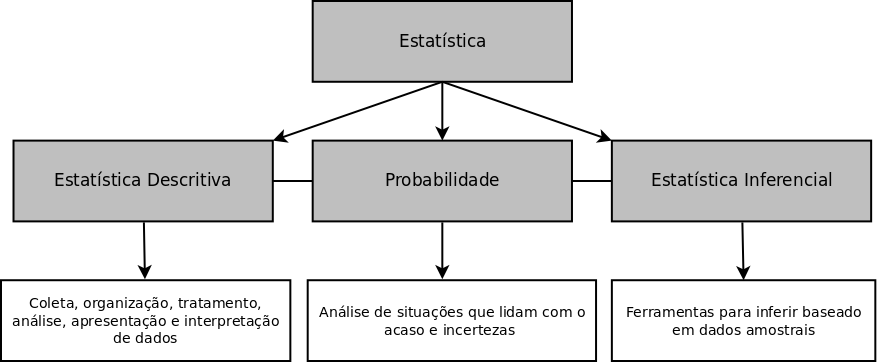
\includegraphics[width=1\textwidth]{../img/organograma_estatistica.png}
  \end{figure}
\end{frame}

\begin{frame}{Áreas da Estatística}
  \textbf{Estatística Descritiva}: etapa inicial de qualquer análise. É
  um conjunto de técnicas destinadas a descrever e resumir os dados, que
  auxiliam a descrever características de interesse.\\
  $\Rightarrow$ ``\textit{Conheça seus dados}'' \\~\\
  \textbf{Probabilidade}: é a ferramenta matemática utilizada pela
  Estatística para se estudar a \textbf{incerteza} oriunda de fenômenos
  \textbf{aleatórios}. \\
  $\Rightarrow$ ``\textit{Qual a incerteza associada aos dados?}'' \\~\\
  \textbf{Estatística Inferencial}: é um conjunto de técnicas que
  possibilita tirar conclusões sobre uma \textbf{população}, a partir de
  um subconjunto de valores (\textbf{amostra}). \\
  $\Rightarrow$ ``\textit{Quais conclusões podemos tirar a partir destes
    dados?}''
\end{frame}

\section[Amostragem]{Conceitos de amostragem}

\begin{frame}{Conceitos de amostragem}
  Quando fazemos uma pesquisa, ou utilizamos algum mecanismo para obter
  informações, um dos objetivos principais é \textbf{coletar dados de
    uma pequena parte} de um \textsl{grande grupo} e
  \underline{aprender} então alguma coisa sobre esse grupo maior
\end{frame}

\begin{frame}{População e amostra}
  \begin{figure}[h]
    \centering
    \includegraphics[width=.9\textwidth]{../img/populacao_amostra.png}
  \end{figure}
\end{frame}

\begin{frame}{Conceito de amostragem}
  \begin{center}
    ``Astros do rock morrem jovens.''
  \end{center}
  \begin{figure}[h]
    \centering
    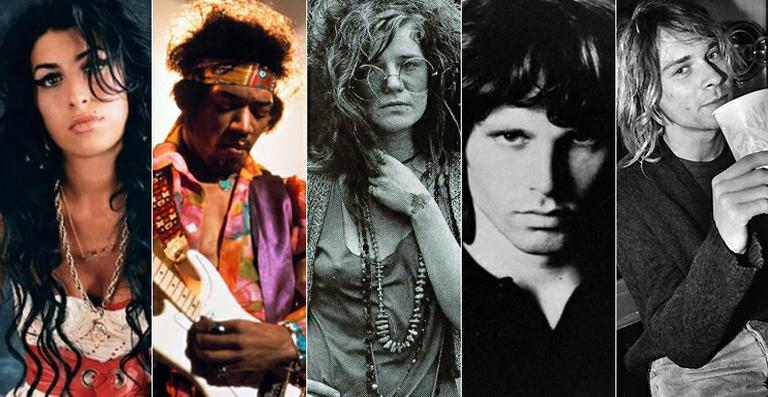
\includegraphics[width=.8\textwidth]{../img/rock}
  \end{figure}
  \begin{center}
    Todos os astros do rock morrem jovens?
  \end{center}
\end{frame}

\begin{frame}{População e amostra}
  \textbf{População}: conjunto de indivíduos, objetos ou produtos que
  contém a característica que temos interesse. Exemplo:
  \begin{itemize}
  \item Característica: altura dos estudantes da UFPR
  \item População: \textbf{todos} os estudantes da UFPR
  \end{itemize}
  \begin{alertblock}{Observação}
    A população depende do interesse da pesquisa
  \end{alertblock}
  \vspace{1em}
  \textbf{Amostra}: subconjunto da população, em geral com dimensão bem
  menor, que também possui a característica de interesse. Exemplo:
  \begin{itemize}
  \item Característica: altura dos estudantes da UFPR
  \item Amostra: 100 estudantes selecionados \textbf{ao acaso}
  \end{itemize}
\end{frame}

\begin{frame}{Parâmetro e Estatística}
  \begin{center}
    População $\rightarrow$ \textbf{censo} $\rightarrow$
    \textbf{parâmetro} \\~\\
    \textsl{Uma medida numérica que descreve alguma
      característica da \underline{população}, usualmente representada
      por letras gregas: $\theta$, $\mu$, $\sigma$, $\ldots$} \\~\\
    Exemplo: média populacional = $\mu$
  \end{center}
  \vspace{1em}
  \hrule
  \vspace{1em}
  \begin{center}
    População $\rightarrow$ \textbf{amostra} $\rightarrow$
    \textbf{estatística}  \\~\\
    \textsl{Uma medida numérica que descreve alguma
      característica da \\ \underline{amostra}, usualmente denotada pela
    letra grega do respectivo parâmetro com um acento circunflexo:
    $\hat\theta$, $\hat\mu$, $\hat\sigma$, $\ldots$} , ou por letras do
  alfabeto comum: $\bar x$, $s$, $\ldots$\\~\\
    Exemplo: média amostral = $\bar{x}$
  \end{center}
\end{frame}

% \begin{frame}{Estimador e estimativa}
%   \textbf{Estimador:}
% \end{frame}

\begin{frame}{Exemplo}
  \begin{itemize}
  \item População: todos os alunos de uma única turma
  \item Característica: idade dos alunos
    \vspace{1em}
  \end{itemize}
  Censo: \texttt{22 21 24 23 20 22 21 25 24 24 23 19
    25 24 23 23 20 21 23 20 23
    22 23 23 25 25 20 23 24 20}
  \begin{center}
    Média populacional: $\mu = 22,5$ $\quad \Leftarrow \quad$
    \textbf{Parâmetro}
  \end{center}
  Amostra de 5 alunos: \texttt{25 24 23 23 25}
  \begin{center}
    Média amostral: $\bar{x} = 24$ $\quad \Leftarrow \quad$
    \textbf{Estatística}
  \end{center}
\end{frame}

\begin{frame}{Por que fazer amostragem?}
  \begin{itemize}
  \item Parâmetros populacionais desconhecidos
  \item Impossibilidade de realização de um censo
  \item Mais barato, mais rápido
  \end{itemize}\pause
  \begin{alertblock}{Atenção!}
    Não existe nenhuma técnica estatística capaz de salvar uma amostra
    mal coletada!
  \end{alertblock}\pause
  Em geral, uma amostra deve ser
  \begin{itemize}
  \item um subconjunto \textbf{representativo} da população
  \item \textbf{aleatória} (de alguma forma)
  \end{itemize}
%  \vspace{1em}
  Existem diversas maneiras para se \textit{retirar} uma
  \textbf{amostra} de uma \textit{população} $\rightarrow$
  \textbf{Teoria da Amostragem}
\end{frame}

% \begin{frame}{Porque fazer amostragem?}
%   Nota sobre seleção de amostras aleatórias
% \end{frame}

% \subsection{Tipos de estudos}

% \begin{frame}{Tipos de estudos}
%   \begin{block}{Observacional}
%     Observa e mede características, mas \textbf{não modifica} o objeto
%     de estudo.\\~\\
%     Exemplo: Pesquisa da idade ou altura dos alunos da UFPR
%   \end{block}\vspace{1em}
%   \begin{block}{Experimental}
%     Aplica um \textbf{tratamento}, e passa a observar seu efeito entre
%     o objeto de estudo.\\~\\
%     Exemplo: Estudo do efeito de um novo medicamento
%   \end{block}
% \end{frame}

% Bussab e Morettin, sec. 10.4
\subsection[Tipos]{Tipos de Amostragem}

\begin{frame}{Tipos de amostragem}
  \begin{block}{(A) Levantamentos amostrais}
    A amostra é obtida a partir de uma população bem definida, bem meio
    de processos bem definidos pelo pesquisador. Subdivide-se em dois
    grupos:
    \begin{description}
    \item[Probabilísticos] Cada elemento da população possui a
    mesma probabilidade se ser selecionado para compor a amostra
    $\rightarrow$ mecanismos aleatórios de seleção
  \item[Não probabilísticos] A seleção da amostra depende do julgamento
    do pesquisador. Há uma \textbf{escolha} deliberada dos elementos
    para compor a amostra $\rightarrow$ mecanismos não aleatórios de
    seleção
    \end{description}
  \end{block}
\end{frame}

\begin{frame}{Tipos de amostragem}
  \begin{block}{(B) Planejamento de Experimentos}
    Aplica um \textbf{tratamento}, e passa a observar seu efeito entre
    o objeto de estudo. Requer, portanto, a interferência do pesquisador
    sobre a população, bem como o controle de fatores externos, com o
    intuito de medir o efeito desejado.\\
    \vspace{1em}
    Exemplos: Estudo do efeito de um novo medicamento, experimentos
    agronômicos
  \end{block}
\end{frame}

\begin{frame}{Tipos de amostragem}
  \begin{block}{(C) Levantamentos Observacionais}
    Observa e mede características, mas \textbf{não modifica} o objeto
    de estudo. Os dados são coletados sem que o pesquisador tenha
    controle sobre as informações obtidas. \\
    \vspace{1em}
    Exemplo: Verificar o valor das vendas de uma empresa em um certo
    período (não há como ``selecionar'' as vendas)
  \end{block}
\end{frame}

\subsection[Métodos]{Métodos de amostragem}

% \begin{frame}{Métodos de amostragem}
%   \begin{block}{Probabilístico}
%     Cada elemento da população possui a mesma probabilidade se ser
%     selecionado para compor a amostra
%   \end{block}
%   \vspace{1em}
%   \begin{block}{Não probabilístico}
%     A seleção da amostra depende do julgamento do pesquisador. Há uma
%     \textbf{escolha} deliberada dos elementos para compor a amostra
%   \end{block}
% \end{frame}

\begin{frame}{Métodos de amostragem}
  Para a escolha do método deve-se levar em conta:
  \begin{itemize}
  \item Tipo de pesquisa
  \item Acessibilidade e disponibilidade dos elementos da população
  \item Disponibilidade de tempo
  \item Recursos financeiros e humanos
  \item \ldots
  \end{itemize}
\end{frame}

\subsubsection{Não probabilísticos}

\begin{frame}{Métodos não probabilísticos}
  Exemplos: \\~\\
  \textbf{Amostragem por conveniência}: elementos selecionados por serem
  imediatamente disponíveis.\\
  Exemplo: Uma repórter entrevistando pessoas na rua \\~\\
  \textbf{Amostragem por julgamento}: uma pessoa experiente no assunto
  \textbf{escolhe} intencionalmente os elementos a serem amostrados. \\
  Exemplo: Novo produto ``testado'' entre funcionários\\~\\
  \pause
  \begin{alertblock}{Atenção}
    Na amostragem não probabilística, os elementos da população não
    tem a mesma probabilidade de serem selecionados, portanto \textbf{não
    há garantias da \underline{representatividade} da população}!
  \end{alertblock}
\end{frame}

\subsubsection{Probabilísticos}

\begin{frame}{Métodos probabilísticos}
  \begin{block}{Amostragem Aleatória Simples (AAS)}
    Todas as possíveis amostras de tamanho $n$ tem a mesma chance de
    serem escolhidas (de uma população com $N$ elementos)
  \end{block}
  \textbf{Exemplos}:
  \begin{itemize}
  \item Selecionar 10 estudantes de uma sala \textbf{por sorteio} e
    perguntar a idade
  \item Gerar uma amostra aleatória de 1000 números de matrícula de
    estudantes da UFPR (no computador!) e perguntar a idade
  \end{itemize}
\end{frame}

\begin{frame}{Métodos probabilísticos}
  \begin{block}{Amostragem Aleatória Simples (AAS)}
    \begin{itemize}
    \item É o método mais simples para selecionarmos uma amostra
      probabilística de uma população
    \item Serve de base para outros procedimentos amostrais,
      planejamento de experimentos e estudos observacionais
    \item Utilizando-se um procedimento aleatório, sorteia-se um
      elemento da população. Repete-se o  processo até que sejam
      sorteadas as $n$ unidades na amostra.
    \end{itemize}
  \end{block}
\end{frame}

\begin{frame}{Métodos probabilísticos}
%  \textbf{\underline{Tipos de amostragem probabilística}}\vspace{2em}\\
  \begin{block}{Amostragem Aleatória Simples (AAS)}
    \textbf{Com reposição}: o mesmo elemento da população pode ser amostrado
    mais de uma vez. \textsl{A probabilidade de seleção \textbf{não} se
      altera}. \\~\\
    \textbf{Sem reposição}: cada elemento da população é amostrado uma
    única vez. \textsl{A probabilidade de seleção se altera}.
  \end{block}
  \begin{alertblock}{Atenção!}
    Na prática, em populações \textit{infinitas} (muito grandes), a
    reposição ou não é irrelevante
  \end{alertblock}
\end{frame}

\begin{frame}{Métodos probabilísticos}
  \begin{block}{Amostragem Aleatória Simples (AAS)}
    Do ponto de vista da quantidade de informação contida na amostra,
    a amostragem \textsl{sem reposição} é mais adequada. \\~\\
    No entanto, a amostragem \textsl{com reposição} conduz a um
    tratamento teórico mais simples, pois ele implica que tenhamos
    \textbf{independência} entre as unidades selecionadas. \\~\\
    Portanto, na maioria dos casos quando nos referenciarmos a uma AAS,
    estamos nos referenciando a uma \textbf{amostragem aleatória simples
    com reposição}.
  \end{block}
\end{frame}

\begin{frame}{Métodos probabilísticos}
  \begin{block}{Amostragem sistemática}
    Utilizada quando os elementos estão dispostos de maneira organizada
    (ex.: fila, lista) e \textbf{aleatória}.\\
    Escolhe um ponto de partida e seleciona-se cada $k$-ésimo elemento
    da população (ex.: o 50$^{\circ}$ elemento)
  \end{block}
  \textbf{Exemplo}:
  \begin{itemize}
  \item Em uma fábrica de lâmpadas, a cada 100 peças produzidas, uma é
    retirada para teste
  \end{itemize}
\end{frame}

\begin{frame}{Métodos probabilísticos}
  \begin{block}{Amostragem estratificada}
    Indicada quando a população está dividida em grupos distintos,
    denominados \textbf{estratos}.\\
    Dentro de cada estrato é realizada uma amostragem aleatória
    simples. O tamanho da amostra pode ou não ser proporcional ao
    tamanho do estrato.
  \end{block}
  \textbf{Exemplos}:
  \begin{itemize}
  \item Uma comunidade universitária com 8000 indivíduos está
    estratificada da seguinte forma
    \begin{table}[h]
      \centering
      \begin{tabular}{lll}
        \hline
        \textbf{Estrato} & \textbf{População} & \textbf{Amostra} \\ \hline
        Professores & 800 & 80 \\ \hline
        Funcionários & 1200 & 120 \\ \hline
        Estudantes & 6000 & 600 \\
        \hline
      \end{tabular}
    \end{table}
  \end{itemize}
\end{frame}

\begin{frame}{Métodos probabilísticos}
  \begin{block}{Amostragem por conglomerado}
    A área da população é dividida em seções (ou
    \textbf{conglomerados}, ex.: bairros, quarteirões). Os conglomerados
    são selecionados aleatoriamente. Dentro de um conglomerado,
    \textbf{todos} os elementos são amostrados.
  \end{block}
  \textbf{Exemplo}:
  \begin{figure}[h]
    \centering
    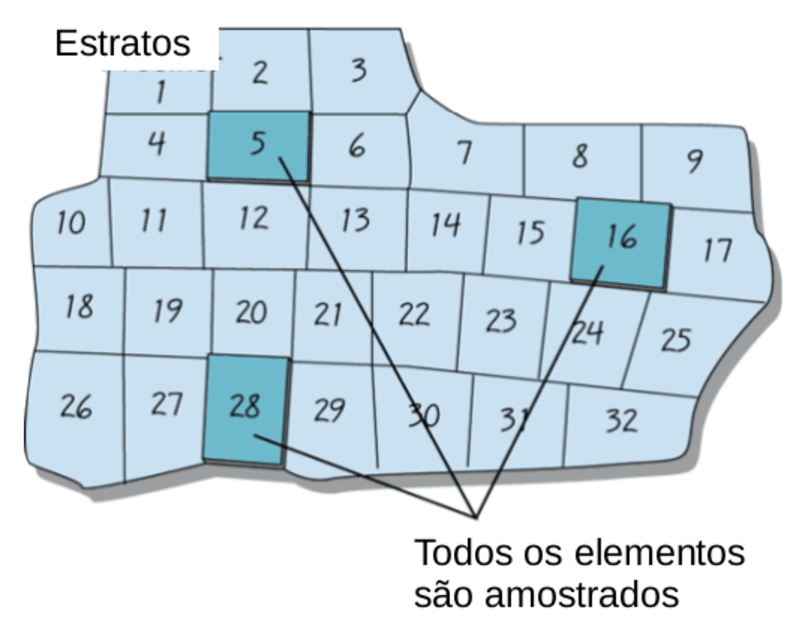
\includegraphics[width=.5\textwidth]{../img/conglomerado2}
  \end{figure}
\end{frame}

\section{Erros amostrais}

\begin{frame}{Erros amostrais}
  \begin{block}{Erros amostrais}
    Diferença entre o resultado da amostra e o verdadeiro valor da
    população. Ocorre pois as amostras são \textbf{aleatórias}!
  \end{block}
  \vspace{1em}
  \begin{block}{Erros não amostrais}
    Ocorre quando os dados amostrais são coletados
    \textbf{incorretamente}, devido a uma \textsl{amostra tendenciosa},
    instrumento de medida defeituoso, anotações erradas, \ldots
  \end{block}
  \pause
  \begin{alertblock}{Atenção!}
    Os erros não amostrais não devem existir, ou devem ser minimizados
  \end{alertblock}
\end{frame}

\begin{frame}{Erros amostrais}
  Não importa quão bem a amostra seja coletada, os \textbf{erros
    amostrais} sempre irão ocorrer\\~\\
  Cada vez que uma amostra aleatória for retirada de uma população, um
  resultado diferente será observado\\~\\
  Selecione uma amostra de tamanho $n = 5$ das idades dos estudantes de
  uma sala: \texttt{22 21 24 23 20 22 21 25 24 24 23 19
    25 24 23 23 20 21 23 20 23
    22 23 23 25 25 20 23 24 20}\\~\\
  Repita 5 vezes (tente ser o mais aleatório possível!), calcule a média
  de cada amostra, e compare com a média populacional $\mu = 22,5$
\end{frame}


\begin{frame}{Um exemplo}
  \begin{table}[h]
    \centering
    \begin{tabular}{lrr}
      \hline
      Amostra & $\bar{x}$ & $\epsilon = \bar{x} - \mu$ \\
      \hline
      23 23 23 24 23 & 23.2 & 0.7 \\
      24 22 20 20 20 & 21.2 & -1.3 \\
      21 20 19 22 25 & 21.4 & -1.1 \\
      22 23 25 20 22 & 22.4 & -0.1 \\
      21 20 22 24 20 & 21.4 & -1.1 \\
      \hline
    \end{tabular}
  \end{table}
  \begin{itemize}
  \item O que isso nos diz a respeito das médias amostrais?
  \item O que isso nos diz a respeito da variabilidade das médias
    amostrais?
  \item E se fizemos uma ``\underline{média das médias}'' de todas as
    amostras?
  \end{itemize}
  Voltaremos aqui mais tarde \ldots
\end{frame}

% \begin{frame}{População e amostra}
%   \textbf{População}: conjunto de indivíduos, objetos ou produtos que
%   contém a característica que temos interesse. Exemplo:
%   \begin{itemize}
%   \item Característica: altura dos estudantes da UFPR
%   \item População: \textbf{todos} os estudantes da UFPR
%   \end{itemize}
%   \vspace{2em}
%   \textbf{Amostra}: subconjunto da população, em geral com dimensão bem
%   menor, que também possui a característica de interesse. Exemplo:
%   \begin{itemize}
%   \item Característica: altura dos estudantes da UFPR
%   \item Amostra: 100 estudantes selecionados \textbf{ao acaso}
%   \end{itemize}
% \end{frame}

% \begin{frame}{População e amostra}
%   \begin{figure}[h]
%     \centering
%     \includegraphics[width=.9\textwidth]{populacao_amostra.png}
%   \end{figure}
% \end{frame}

% \begin{frame}{Métodos de amostragem}
%   Existem diversas maneiras para se \textit{retirar} uma
%   \textbf{amostra} de uma \textit{população}.\\~\\
%   Em geral, uma amostra deve ser
%   \begin{itemize}
%   \item um subconjunto \textbf{representativo} da população
%   \item \textbf{aleatória} (de alguma forma)
%   \end{itemize}
%   \vspace{1em}
%   Os diversos métodos de amostragem fazem parte da \textbf{Teoria da
%     Amostragem}
% \end{frame}

% \begin{frame}{Variáveis}
%   Quando fazemos uma \textbf{amostragem}, coletamos não apenas a
%   informação sobre a característica de interesse, mas \textit{diversas
%     outras informações} que auxiliarão no entendimento desta
%   característica.\\~\\
%   Cada uma das características da população amostrada, como peso,
%   altura, sexo ou idade, é denominada de uma \textbf{variável}\\~\\
%   As \textit{variáveis} podem assumir diferentes valores, que
%   basicamente podem ser separados em
%   \begin{itemize}
%   \item \textbf{Quantitativos} ou numéricos
%   \item \textbf{Qualitativos} ou não numéricos, ou \textit{categóricos}
%   \end{itemize}
% \end{frame}

% \begin{frame}{Classificação de variáveis}
%   As \textbf{variáveis quantitativas} ou numéricas podem ser
%   \begin{itemize}
%   \item \textbf{Discretas}: assumem apenas valores inteiros. Ex.: número
%     de irmãos, número de passageiros
%   \item \textbf{Contínuas}: assume qualquer valor no intervalo dos
%     números reais. Ex.: peso, altura
%   \end{itemize}
%   \vspace{1em}
%   As \textbf{variáveis qualitativas} ou categóricas podem ser
%   \begin{itemize}
%   \item \textbf{Nominais}: quando as categorias não possuem uma ordem
%     natural. Ex.: nomes, cores, sexo.
%   \item \textbf{Ordinais}: quando as categorias podem ser
%     ordenadas. Ex.: tamanho (pequeno, médio, grande), classe social
%     (baixa, média, alta), grau de instrução (básico, médio, graduação,
%     pós-graduação)
%   \end{itemize}
% \end{frame}

% \begin{frame}{Classificação de variáveis}
%   \begin{figure}[h]
%     \centering
%     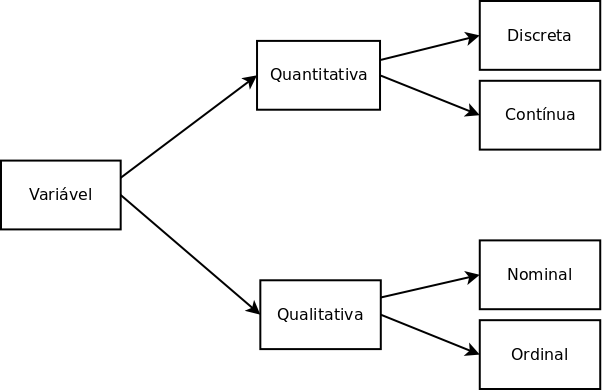
\includegraphics[width=.9\textwidth]{classificacao_variaveis.png}
%   \end{figure}
% \end{frame}

\section{Referências}

\begin{frame}{Referências}
  % \textbf{Referências Básicas}
  \begin{itemize}
  \item Bussab, WO; Morettin, PA. \textbf{Estatística básica}. São
    Paulo: Saraiva, 2002. 526 p. [Cap. 1 e 10]
  \item Magalhães, MN; Lima, ACP. \textbf{Noções de Probabilidade e
      Estatística}. São Paulo: EDUSP, 2008. [Cap. 1]
  % \end{itemize}
  % \textbf{Referências Complementares}
  % \begin{itemize}
  \end{itemize}
\end{frame}

\end{document}
